\documentclass[a4paper]{report}
\usepackage[utf8]{inputenc}
\usepackage[T1]{fontenc}
\usepackage{RJournal}
\usepackage{amsmath,amssymb,array}
\usepackage{booktabs}


% tightlist command for lists without linebreak
\providecommand{\tightlist}{%
  \setlength{\itemsep}{0pt}\setlength{\parskip}{0pt}}

\usepackage{longtable}

% Always define CSL refs as bib entries are contained in separate doc
% Pandoc citation processing
%From Pandoc 3.1.8
% definitions for citeproc citations
\NewDocumentCommand\citeproctext{}{}
\NewDocumentCommand\citeproc{mm}{%
  \begingroup\def\citeproctext{#2}\cite{#1}\endgroup}
\makeatletter
 % allow citations to break across lines
 \let\@cite@ofmt\@firstofone
 % avoid brackets around text for \cite:
 \def\@biblabel#1{}
 \def\@cite#1#2{{#1\if@tempswa , #2\fi}}
\makeatother
\newlength{\cslhangindent}
\setlength{\cslhangindent}{1.5em}
\newlength{\csllabelwidth}
\setlength{\csllabelwidth}{3em}
\newenvironment{CSLReferences}[2] % #1 hanging-indent, #2 entry-spacing
 {\begin{list}{}{%
  \setlength{\itemindent}{0pt}
  \setlength{\leftmargin}{0pt}
  \setlength{\parsep}{0pt}
  % turn on hanging indent if param 1 is 1
  \ifodd #1
   \setlength{\leftmargin}{\cslhangindent}
   \setlength{\itemindent}{-1\cslhangindent}
  \fi
  % set entry spacing
  \setlength{\itemsep}{#2\baselineskip}}}
 {\end{list}}
\usepackage{calc}
\newcommand{\CSLBlock}[1]{#1\hfill\break}
\newcommand{\CSLLeftMargin}[1]{\parbox[t]{\csllabelwidth}{#1}}
\newcommand{\CSLRightInline}[1]{\parbox[t]{\linewidth - \csllabelwidth}{#1}\break}
\newcommand{\CSLIndent}[1]{\hspace{\cslhangindent}#1}


%\newcommand{\doi}[1]{\href{https://doi.org/#1}{\normalfont\texttt{doi:\discretionary{}{}{}{#1}}}}


\begin{document}


%% do not edit, for illustration only
\sectionhead{Contributed research article}
\volume{16}
\volnumber{1}
\year{2024}
\month{March}
\setcounter{page}{5}

\begin{article}
  % !TeX root = RJwrapper.tex
\title{Remembering Friedrich ``Fritz'' Leisch}


\author{by Bettina Grün, Kurt Hornik, Torsten Hothorn, Theresa Scharl, and Achim Zeileis}

\maketitle

\abstract{%
This article remembers our friend and colleague Fritz Leisch (1968--2024) who sadly died earlier this year. Many of the readers of The R Journal will know Fritz as a member of the R Core Team and for many of his contributions to the R community. For us, the co-authors of this article, he was an important companion on our journey with the R project and other scientific endeavours over the years. In the following, we provide a brief synopsis of his career, present his key contributions to the R project and to the scientific community more generally, acknowledge his academic service, and highlight his teaching and mentoring achievements.
}

\section{Career}\label{career}

Friedrich Leisch (see Figure~\ref{fig:leisch}) was born 1968 in Vienna (Austria) and
died after serious illness in 2024 in Vienna. Everyone called him Fritz.

\begin{figure}[h!]

{\centering 
\includegraphics[width=0.55\linewidth]{figures/img-leisch} 

}

\caption{Fritz Leisch at his inaugural lecture at BOKU in 2011. Source: BOKU.}\label{fig:leisch}
\end{figure}

Starting in 1987, Fritz studied Applied Mathematics at Technische Universität Wien (TU Wien),
earning his master's degree (Dipl.-Ing.) in 1993. Subsequently, he joined the
Department of Statistics and Probability Theory at TU Wien as an
assistant professor which he continued to be, with short intermissions, until 2006.
During this time he also defended his doctoral thesis in Applied Mathematics (Dr.techn.)
in 1999 and earned his habilitation (venia docendi) in Statistics in 2005.

In 1995, he visited the Knowledge-Based Engineering Systems Group at the University of
South-Australia in Adelaide on a Kurt Gödel scholarship for postgraduate
studies. From 1997 to 2004 he was a member of the SFB project
``Adaptive Information Systems and Modeling in Economics and Management Science'', coordinated
at Wirtschaftsuniversität Wien (WU Wien). From 2002 to 2003 he was assistant professor
at the Department of Statistics and Decision Support Systems, Universität Wien.

In 2006 Fritz moved to Munich, Germany, to become a professor for computational
statistics at the Department of Statistics, Ludwig-Maximilians-Universität München (LMU), see Figure~\ref{fig:lmu}.
He returned to Vienna in 2011 to join the BOKU University as head of the Institute of Statistics, see Figure~\ref{fig:boku}.

\begin{figure}[t!]

{\centering 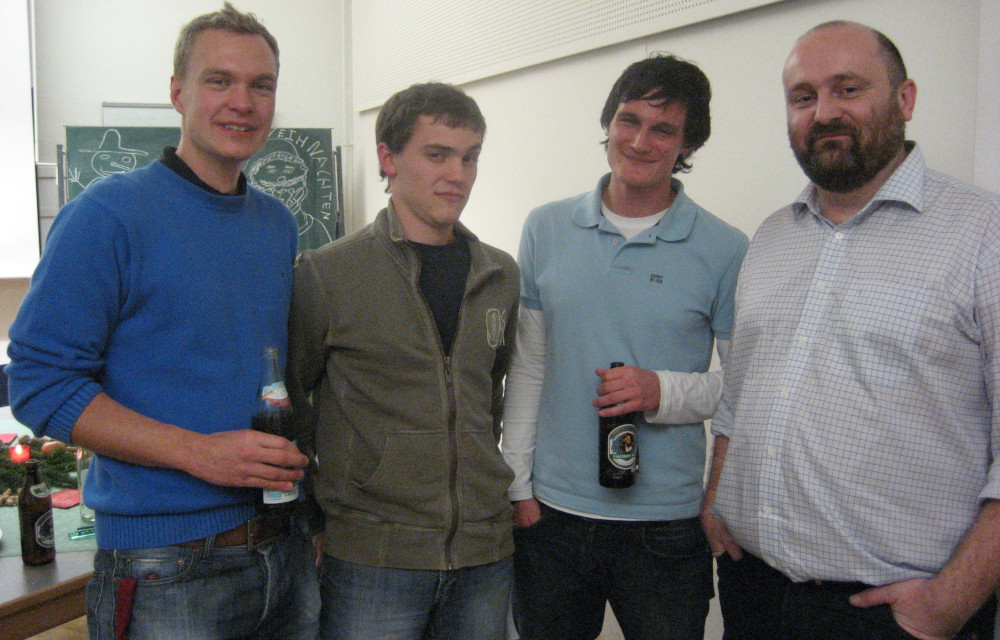
\includegraphics[width=0.83\linewidth]{figures/img-lmu} 

}

\caption{Computational statistics group at LMU in 2007 (left to right): Sebastian Kaiser, Adrian Duffner, Manuel Eugster, Fritz Leisch. Source: Carolin Strobl.}\label{fig:lmu}
\end{figure}

\begin{figure}[t!]

{\centering 
\includegraphics[width=0.83\linewidth]{figures/img-boku} 

}

\caption{Institute of Statistics at BOKU in 2022 (left to right, back to front): Johannes Laimighofer, Nur Banu Özcelik, Ursula Laa, Fritz Leisch, Bernhard Spangl, Gregor Laaha, Matthias Medl. Robert Wiedermann, Lena Ortega Menjivar, Theresa Scharl, Melati Avedis. Source: BOKU.}\label{fig:boku}
\end{figure}

\section{Key contributions}\label{key-contributions}

Fritz' scientific contributions span an impressive range including
theoretical and methodological work (especially in the field of clustering
and finite mixture models) over software (mostly related to the R
programming language) to applied work and cooperations (notably in
marketing, biotechnology, and genomics, among many others). In the
following sections we try to highlight his key contributions and
scientific legacy.

\subsection{R Core \& CRAN}\label{r-core-cran}

During his stay in Australia, Fritz had learned about the existence of
R. Back in Austria, he and Kurt started to explore this potentially
good news more systematically. They soon stopped further work on a
statistics toolbox they had developed for Octave \citep{Eaton+Bateman+Hauberg:2024},
and switched to R for their applied work, finding lots of room for
further improvement, and thus sending polite emails with patches and
more suggestions to Ross Ihaka and Robert Gentleman. Clearly these were
acceptable in quality but too high in quantity, and it did not take very
long that Ross and Robert gave Fritz and Kurt write access to the R
sources (initially in CVS, then moved to SVN), and in 1997, they both
officially became very early members of the R Core Team.

One of the main challenges then was that the functionality provided by R
was rather limited. Contributed extensions for S were available from the
Carnegie Mellon University Statlib S Archive\footnote{Unfortunately, the Statlib
  S Archive is currently not available anymore. A snapshot, including many
  of the actual source code files, is available on the Internet Archive at
  \url{https://web.archive.org/web/20000815063825/http://lib.stat.cmu.edu/S/}.}, and could typically be
ported to R rather easily, but there was no mechanism for conveniently
distributing or actually using these extensions. This fundamentally
changed, when in 1997 Fritz and Kurt implemented the R package
management system, using ideas from Debian's APT (advanced package tool,
\url{https://wiki.debian.org/AptCLI}) they had successfully employed for
managing their computer systems. They also set up the Comprehensive R
Archive Network \citep[CRAN, \url{https://CRAN.R-project.org/}, see also][]{Hornik:2012} as a means for redistributing R and its contributed
extensions, and infrastructure for quality assurance of these
extensions. These two contributions paved the way for the amazing
growth and success of R through its wealth of high-quality contributed
extensions.
See \url{https://stat.ethz.ch/pipermail/r-announce/1997/000001.html} for
the first announcement of CRAN, starting with 12 extension packages.
Currently, there are more than 21,000. See Figure~\ref{fig:cran}
for a screenshot\footnote{This is from the earliest capture, from 1998-01-10,
  available on the Internet Archive at
  \url{https://web.archive.org/web/19980110082558/http://www.ci.tuwien.ac.at/R/contents.html}.}
of the landing page of the CRAN master site at TU Wien, as last modified
by Fritz on 1997-12-09.

\begin{figure}[t!]

{\centering 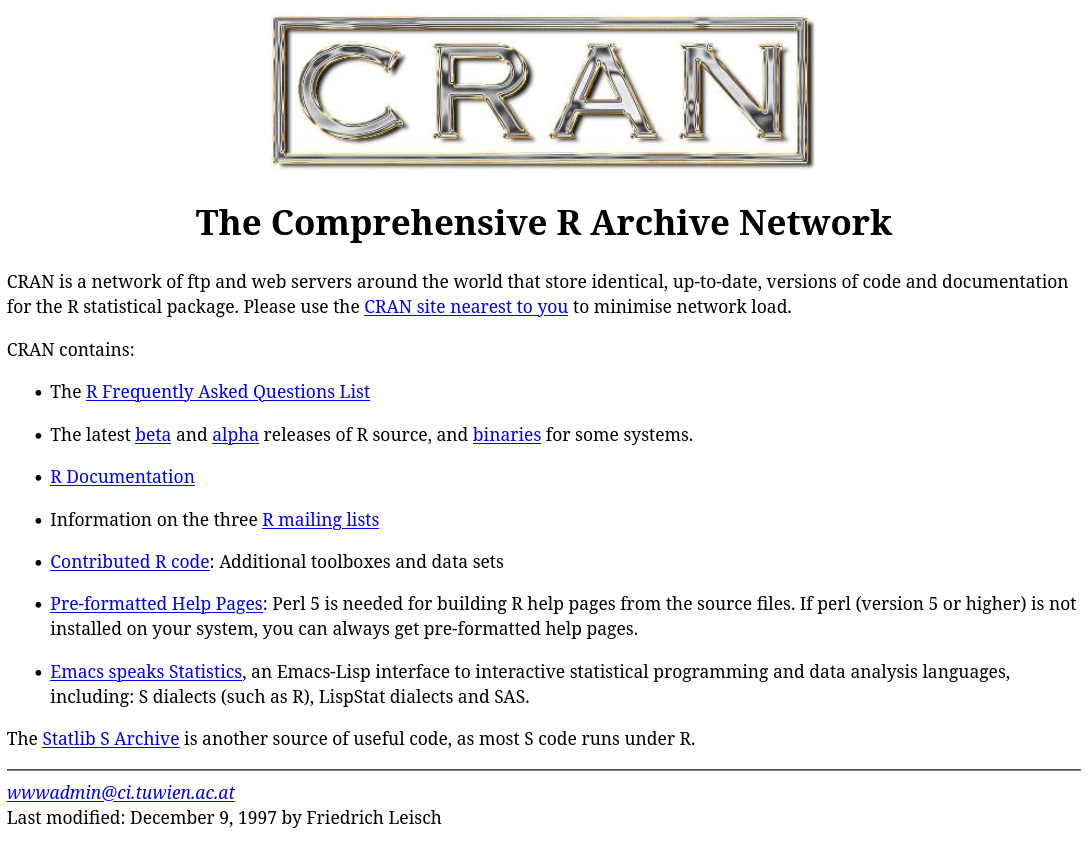
\includegraphics[width=1\linewidth]{figures/img-cran} 

}

\caption{Screenshot of the landing page of the CRAN master site at TU Wien on 1998-01-10, as last modified by Fritz on 1997-12-09. Source: Internet Archive.}\label{fig:cran}
\end{figure}

The first SVN commit by Fritz is from 1997-10-02, the last from
2013-10-04. Overall, there are 651 commits by Fritz, mostly from the
early years of R Core, and related to the R package management and CRAN
mirror system, and the addition of the \texttt{Sweave} system
(see Section~\hyperref[sec:sweave-reproducibility]{2.3} for more details).

\subsection{DSC \& useR! conferences}\label{dsc-user-conferences}

With establishing CRAN in Vienna at TU Wien, Fritz and Kurt
laid the foundation for a special relationship between Vienna and R that they
characterized as a story of ``love and marriage'' \citep{Hornik+Leisch:2002}. In the decade
after the creation of CRAN a number of seminal R-related meetings took place in Vienna,
co-organized by Fritz as well as several of the co-authors of this paper.

The first workshop on ``Distributed Statistical Computing'' (DSC) took place from
March 19-23, 1999, at TU Wien. The main motivations were bringing together the R Core Team
for its first face-to-face meeting, discussing the roadmap for the release of R 1.0.0,
as well as exploring potential synergies with other environments for statistical computing.
There were around 30 participants and about 20 presentations, many of which were
relatively short, leaving ample time for discussions (see Figure~\ref{fig:dsc1999}).

\begin{figure}[p!]

{\centering 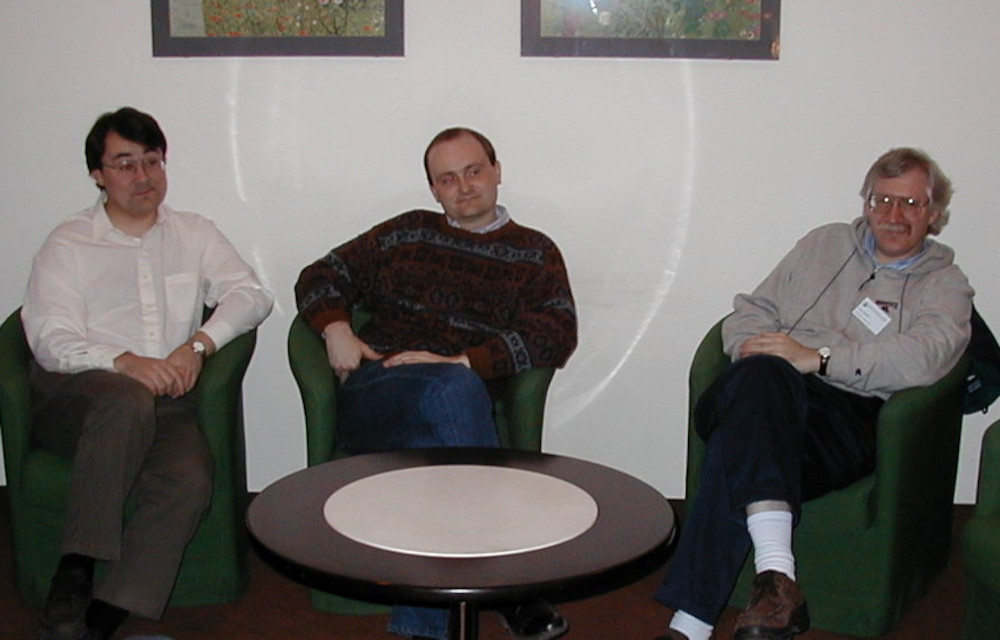
\includegraphics[width=0.83\linewidth]{figures/img-dsc1999a} 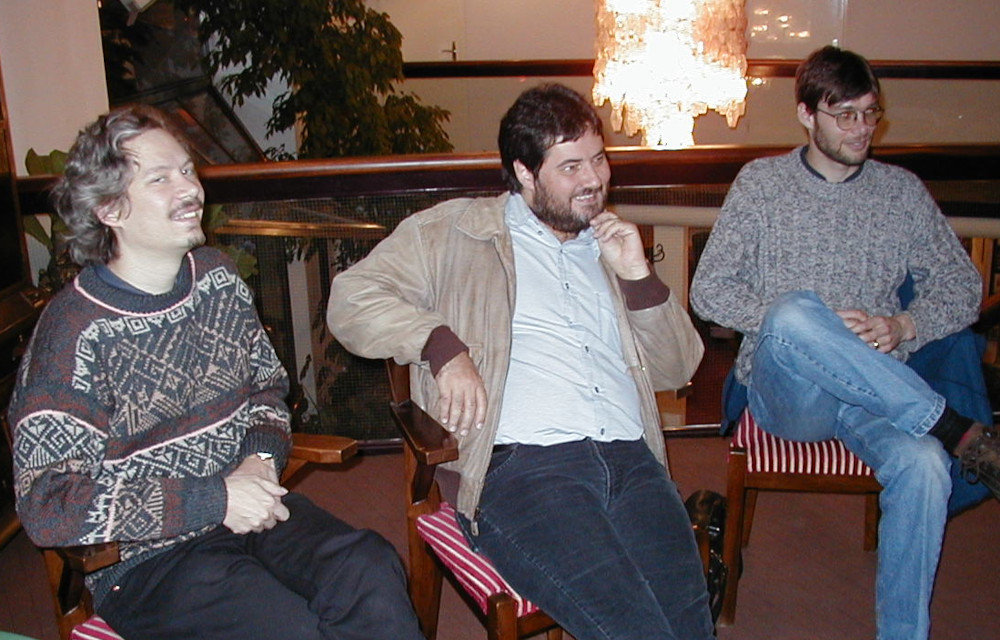
\includegraphics[width=0.83\linewidth]{figures/img-dsc1999b} 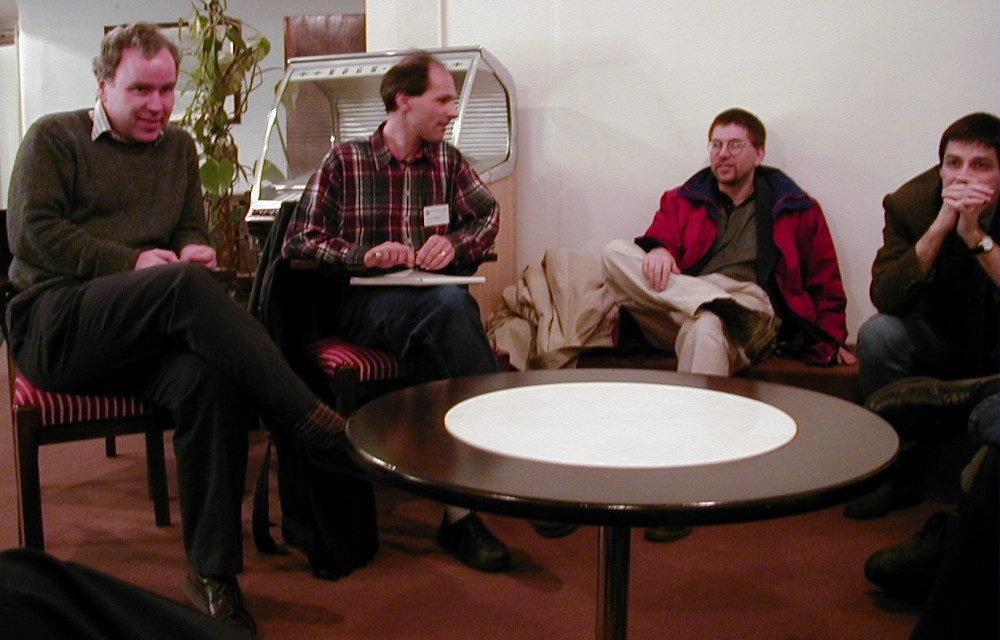
\includegraphics[width=0.83\linewidth]{figures/img-dsc1999c} 

}

\caption{Discussions at DSC 1999 (top to bottom, left to right): Thomas Lumley, Fritz Leisch, Luke Tierney. Peter Dalgaard, Ross Ihaka, Paul Murrell. Brian Ripley, Martin Mächler, Robert Gentleman, Kurt Hornik. Source: Douglas Bates (DSC 1999 homepage).}\label{fig:dsc1999}
\end{figure}

Two more DSC workshops were organized at TU Wien
in 2001 and 2003. While meetings focusing on R development issues (with the
R Core Team and everyone else interested) were still an important part of
these conferences, they also saw an increasing number of regular conference
presentations on R packages and their different fields of application
(e.g., establishing infrastructure for spatial data). In 2001 there were
around 60 participants and about 30 presentations, most with corresponding
papers in the online proceedings \citep{Hornik+Leisch:2001}. In 2003 this
increased to more than 150 participants and about 60 presentations, again
with the majority in the online proceedings \citep{Hornik+Leisch+Zeileis:2003}.

The high demand for a platform, where R users from different fields could
exchange ideas, prompted the creation of a new conference series called
useR!. The first two installments again took place in Vienna in 2004
at TU Wien and in 2006 at WU Wien.
Torsten Hothorn, David Meyer, and Achim Zeileis took the lead in the
organization with support and advice from Fritz and Kurt in the background.
An important contribution from the R Core Team at the useR! conferences
were keynote lectures highlighting important developments, e.g., a keynote
given by Fritz at useR! 2004 on S4 classes and methods. Both conferences
continued the success of the earlier DSC workshops with the number of
participants rising to more than 200 in 2004 and close to 350 in 2006.
Similarly, the number of presentations grew to about 100 in 2004 and more
than 150 in 2006.

In addition to the efforts initiated by Fritz and Kurt, another key factor
to the success of these meetings was the city of Vienna with its culture,
cafes, wine and beer pubs, etc. \citep[see][ and also
Figure~\ref{fig:user2006}]{Hornik+Leisch:2002}.

\begin{figure}[t!]

{\centering 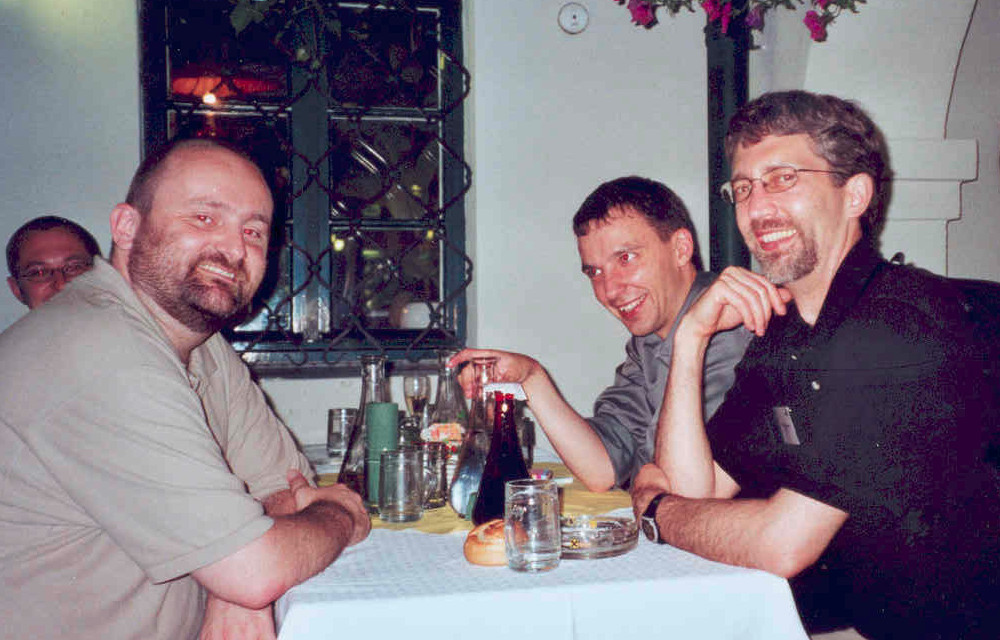
\includegraphics[width=0.83\linewidth]{figures/img-user2006} 

}

\caption{Conference dinner at useR! 2006 (left to right): Fritz Leisch, Torsten Hothorn, Tim Hesterberg. Source: Carolin Strobl (useR! 2006 homepage).}\label{fig:user2006}
\end{figure}

\subsection{Sweave \& reproducibility}\label{sweave-reproducibility}

With \texttt{Sweave} \citep{Leisch:2002}, Fritz pioneered what we now can understand as
the technical foundation of reproducible research. \texttt{Sweave} was the main
inspiration for \CRANpkg{knitr} \citep{Xie:2015} which in turn led to
\CRANpkg{rmarkdown} \citep{Xie+Allaire+Grolemund:2018} and \CRANpkg{quarto}
\citep{Scheidegger+Teague+Dervieux:2024}. All these systems are used today to
generate countless scientific articles, package vignettes, webpages, books, blogs,
and much more in a dynamic and reproducible way.

Of course, Fritz was not the first one going in this direction. The concept
of ``literate programming'' had been introduced by \citet{Knuth:1984}, allowing to
combine the source code for software and the corresponding documentation
in the same file. The concepts of ``tangling'', that is, extracting the code
for compilation, and ``weaving'', the process of generating a nicely looking
document containing code next to prosa and formulae, have their roots in the
\texttt{WEB} and \texttt{CWEB} systems \citep{Knuth+Levy:1993}. As these packages were specific
to code in Pascal (\texttt{WEB}) and C (\texttt{CWEB}), respectively, and documentation in
LaTeX, \citet{Ramsey:1994} introduced his \texttt{noweb} system as a literate programming
tool that is agnostic to the programming language used and also supports HTML
in addition to LaTeX and a few other backends for documentation. The \texttt{noweb}
syntax for code chunks is:

\pagebreak

\begin{verbatim}
<<code>>=
1 + 2
@
\end{verbatim}

This will look familiar to users of \texttt{Sweave}. From this history, the naming
decisions for the software and its file format can be understood: \texttt{Sweave}
is the function that weaves code in S (or R - both languages still existed
side by side at the time) with its output and documentation. And \texttt{Rnw} stands for files
mixing R code with \texttt{noweb} syntax.

Starting in the mid-1990s to the early 2000s, interests shifted from just
``literate programming'' to ``literate data analysis'' \citep{Leisch:2002, Leisch+Rossini:2003}
as a core ingredient for reproducible research \citep{Buckheit+Donoho:1995}.
The seminal new idea was to have dynamic documents so \emph{outputs} of code
such as figures and tables could be updated automatically when the underlying
data changed, which was pioneered by the late Günter Sawitzki in his
\texttt{Voyager} system \citep{Sawitzki:1996}.

Fritz amalgamated all of this into \texttt{Sweave} which was the first time that the
power of dynamic reporting became easily available in a widely-used programming
language for statistics in combination with the standard textprocessing system
LaTeX. This turned out to be a ``killer feature'' of R at the time and the basis
for further work towards reproducible research \citep{Hothorn+Leisch_2011, Stodden:2014}.

\texttt{Sweave} was also the basis for R package vignettes \citep{Leisch:2003} as an
addition to the previously available technical manual pages.
The first R package vignette published on CRAN in May 2002 was in the
\CRANpkg{strucchange} package, providing methods for testing, monitoring,
and dating structural changes. The vignette was the \texttt{Sweave} adaptation
of an introduction to the package that had been co-authored by Fritz and
published a couple of months earlier in the \emph{Journal of Statistical Software}
\citep{Zeileis+Leisch+Hornik:2002}. See Figure~\ref{fig:sweave} for how
Fritz used it to illustrate the idea of package vignettes in \citet{Leisch:2003}
and that the R code from vignettes can be easily extracted (also interactively),
explored, and re-run.

\begin{figure}[t!]

{\centering 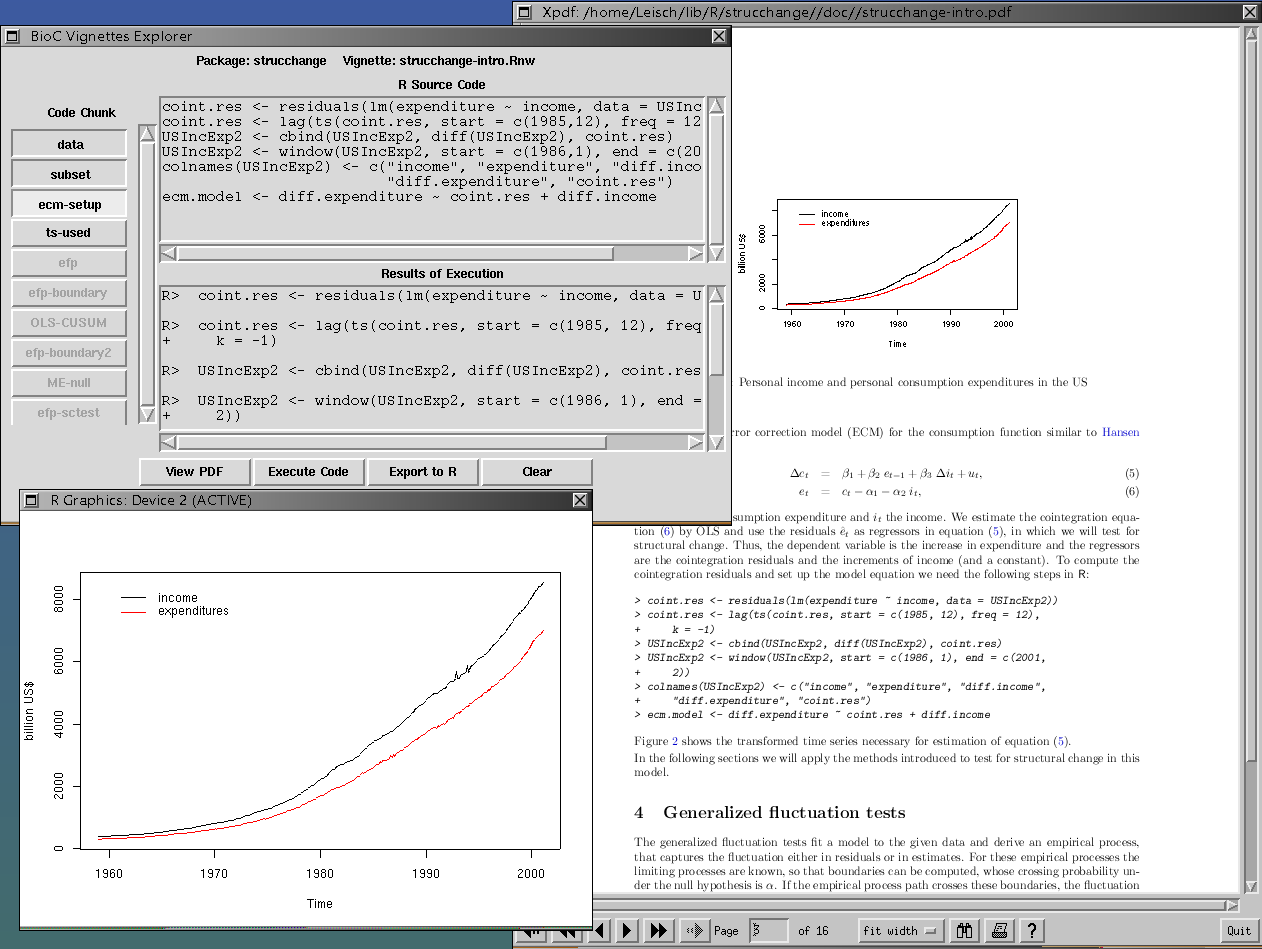
\includegraphics[width=1\linewidth]{figures/img-sweave} 

}

\caption{Screenshot of the strucchange package vignette, shown in a PDF viewer (right), along with the vExplorer from Bioconductor for interactive code execution (top left) with output in the active R graphics window (bottom left). Source: Leisch (2003, Figure 2).}\label{fig:sweave}
\end{figure}

\subsection{Clustering \& mixture models}\label{clustering-mixture-models}

Fritz' theoretical and methodological work focused in particular on
clustering and finite mixture models. Centroid-based partitioning
methods as well as finite mixture models allow that their fitting
algorithm is embedded in a common estimation framework. In this
framework, each of the steps is adapted in a modular way depending on
the specific setup, e.g., the distance and centroid determining method
or the component distribution used. Fritz exploited this for the
implementation of the packages \CRANpkg{flexclust} \citep{Leisch:2006} and
\CRANpkg{flexmix} \citep{Leisch:2004, Gruen+Leisch:2008}, contributing to
the clustering tools available for R (see the CRAN Task View
\ctv{Cluster}). Both packages provide general infrastructure for
(model-based) clustering and enable rapid prototyping and the simple
extension to new variants taking into account complicated data
structures or challenging model specifications \citep[see, for example,
\pkg{psychomix},][]{Frick+Strobl+Leisch:2012}.

\subsection{Applied work}\label{applied-work}

For many years, Fritz and Kurt actively participated in the Biological
Psychiatry working group at Medizinische Universität Wien. The first
paper co-authored by Fritz dates from 2000
\citep{Bailer+Leisch+Meszaros:2000}, the last from 2023
\citep{Solmi+Thompson:2023}. The joint research was mostly
focused on linking genetic traits to psychiatric disorders and
treatment success. This prompted many enhancements in the classical test
infrastructure in base R - in surprising ways to some reviewers, who
could not believe that Fisher's test really worked for tables with more
than two rows or columns. It also established a strong need for
conveniently reporting the results of the statistical analyses to the
medical doctors in the group that went beyond providing annotated
transcripts, which Fritz eventually managed to satisfy by inventing the
\texttt{Sweave} system (see Section~\hyperref[sec:sweave-reproducibility]{2.3}).

Fritz also intensively collaborated with Sara Dolnicar to advance data
analytic methods for data-driven market segmentation analysis. They
received the Charles R. Goeldner Article of Excellence Award for their
work on extracting stable Winter tourist segments in Austria with
bagged clustering \citep{Dolnicar+Leisch:2003}. They focused on the
evaluation of data structure and the selection of suitable segments
based on segment stability as a key criterion \citep{Dolnicar+Leisch:2010, Dolnicar+Leisch:2017}. Finally, this joint work resulted in
\citet{Dolnicar+Gruen+Leisch:2018} which provides practical guidance for
users of market segmentation solutions and for data analysts with
respect to the technical and statistical aspects of market
segmentation analysis.

As head of the Institute of Statistics, Fritz was involved
in various interdisciplinary research projects covering almost the whole
range of core areas of research at BOKU. He was key researcher at the
Austrian Centre of Industrial Biotechnology (acib)
\citep{Scharl+Voglhuber+Leisch:2009, Melcher+Scharl+Leisch:2017} and
faculty member of the doctoral schools on agricultural genomics and
bioprocess engineering. Among others he contributed to the fields of
zoology \citep{Cech:2022}, forestry, transportation and tourism
\citep{Taczanowska:2023} as well as chemistry, genomics and wildlife
biology \citep{Steiner:2014}.

\section{Academic service}\label{academic-service}

In addition to the services for the various conferences and proceedings
already described above, he served the scientific community in various ways.
In January 2001, he co-created \emph{R News} which evolved into
\emph{The R Journal} eight years later. For the journal \emph{Computational Statistics}
he was an associate editor from 2005 to 2006 before he became editor-in-chief
from 2007 to 2011 \citep[see][ for more details]{Symanzik+Mori+Vieu:2024}.
Other notable contributions include being
editor for the \emph{Journal of Statistical Software}, core member of the
\emph{Bioconductor} project for statistical software in bioinformatics, and
first secretary general of the \emph{R Foundation for Statistical Computing} when
it was formed in 2002.

\section{Teaching \& mentoring}\label{teaching-mentoring}

Fritz taught generations of students at bachelor, master, and PhD level and
introduced hundreds of useRs to proper R development in his ``Introduction to
R Programming'' short course. At TU Wien, LMU, and BOKU, he taught courses in applied
statistics, statistical computing and computational statistics. He had the
ability to explain even difficult content in a simple way and to inspire students
with statistics and programming with R. He
co-founded the ``Munich R Courses'' lecture series and was part of a group
aiming to initiate a formal PhD program in statistics at LMU.

Fritz supervised
Bettina Grün, Theresa Scharl,
Sebastian Kaiser, Manuel Eugster,
Christina Yassouridis, Rainer Dangl,
Weksi Budiaji, Muhammad Atif and
Simona Jokubauskaite as his PhD students.
Based on his research, Fritz often discussed the state of and the need for reproducible
research and taught his many students how to avoid the many small and
innocent errors that have a tendency to pile up and invalidate reported
statistical results, with potentially devastating consequences, as we all know.

\section{Odds \& ends}\label{odds-ends}

Fritz loved cooking, music, motorbike riding, playing cards with his
friends, skiing and hiking. A late afternoon call to his office
asking him to go along for a beer in Munich's English Garden almost never went
unanswered, positively. Back in Vienna at BOKU, colleagues got to know Fritz as a very
structured, thoughtful, calm person who involved everyone, listened to
everyone and always endeavored to balance interests and ensure fairness.
He strengthened cooperation and cohesion with his leadership style.
Fritz was a friendly, always modest person who was free of airs and graces or
vanity, despite or perhaps because of his great scientific successes.
The R Core Team and the R community at large miss a contributor,
collaborator, teacher, colleague, and friend.

\bibliography{fritz.bib}

\address{%
Bettina Grün\\
WU Wirtschaftsuniversität Wien\\%
Austria\\
%
%
\textit{ORCiD: \href{https://orcid.org/0000-0001-7265-4773}{0000-0001-7265-4773}}\\%
\href{mailto:Bettina.Gruen@wu.ac.at}{\nolinkurl{Bettina.Gruen@wu.ac.at}}%
}

\address{%
Kurt Hornik\\
WU Wirtschaftsuniversität Wien\\%
Austria\\
%
%
\textit{ORCiD: \href{https://orcid.org/0000-0003-4198-9911}{0000-0003-4198-9911}}\\%
\href{mailto:Kurt.Hornik@R-project.org}{\nolinkurl{Kurt.Hornik@R-project.org}}%
}

\address{%
Torsten Hothorn\\
Universität Zürich\\%
Switzerland\\
%
%
\textit{ORCiD: \href{https://orcid.org/0000-0001-8301-0471}{0000-0001-8301-0471}}\\%
\href{mailto:Torsten.Hothorn@R-project.org}{\nolinkurl{Torsten.Hothorn@R-project.org}}%
}

\address{%
Theresa Scharl\\
BOKU University\\%
Austria\\
%
%
\textit{ORCiD: \href{https://orcid.org/0000-0001-8850-3312}{0000-0001-8850-3312}}\\%
\href{mailto:Theresa.Scharl@boku.ac.at}{\nolinkurl{Theresa.Scharl@boku.ac.at}}%
}

\address{%
Achim Zeileis\\
Universität Innsbruck\\%
Austria\\
%
\url{https://www.zeileis.org/}\\%
\textit{ORCiD: \href{https://orcid.org/0000-0003-0918-3766}{0000-0003-0918-3766}}\\%
\href{mailto:Achim.Zeileis@R-project.org}{\nolinkurl{Achim.Zeileis@R-project.org}}%
}

\end{article}


\end{document}
